\documentclass[12pt]{article}


\usepackage{geometry}
 \geometry{
 a4paper,
 left=20mm,
 right=20mm,
 top=10mm	
 }

\usepackage{amssymb}
\usepackage[utf8]{inputenc}
\usepackage{graphicx}
\usepackage{amstext}
\usepackage{amsmath}


\newtheorem{theorem}{Definice}


\title{VZD - Lineární regrese, regularizace pomocí hřebenové regrese.}
\author{Vastl Martin}

\begin{document}
\maketitle
\author

\section{Lineární regrese}
Cílem lineární regrese je predikovat hodnotu $Y$ na základě příznaků $X_1, X_2, \ldots, X_p$. Při lineární regresi předpokládáme lineární závislost vysvětlované proměnné na příznacích. 

Z důvodu toho, že tato závislost není perfektní tedy, že nečekáme, že pro stejné příznaky $X_1, X_2, \ldots, X_p$ nedostaneme stejné $Y$ modelujeme tuto závislost následovně.
\begin{equation}
Y = w_1x_1 + w_2x_2 + \ldots + w_px_p+\varepsilon,
\end{equation}
kde $w_1, w_2, \ldots, w_p$ jsou nějaké neznáme koeficienty a $\varepsilon$ je náhodná veličina, která není vysvě\-tlitel\-ná za pomocí hodnot příznaků nebo příznaky neznámé nebo cíleně nezahrnované a je tedy z našeho pohledu náhodná.

Obvykle ještě oddělujeme střední hodnotu náhodných vlivů a dostáváme tak:
\begin{equation}
Y = w_0 + w_1x_1 + w_2x_2 + \ldots + w_px_p+\varepsilon,
\end{equation}
kde $E\varepsilon=0$ a $w_0$ se nazývá intercept a odpovídá očekávané výchozí hodnotě při nulových příznacích.

V případě zavedení $x_0=1$ a značení $x=(x_0,x_1,\ldots,x_p)^T$ a $w=(w_0, w_1, \ldots, w_p)^T$ lze zkráceně psát
\begin{equation}
Y = w^Tx+\varepsilon
\end{equation}


Pro konkrétní bod $x$ je skutečná hodnota Y určena vztahem
\begin{equation}
Y = w^Tx+\varepsilon
\end{equation}
a je tedy náhodnou veličinou. Z předpoklad E$\varepsilon=0$ plyne, že E $Y=w^Tx$ a $\hat{Y}$ je tedy bodovým odhadem střední hodnoty E$Y$ v bodě $x$. 
 
\section{Odhad parametrů}
Cílem je nalézt hodnotu vektoru $w$, tak aby byla chyba modelu co nejmenší. Tuto hodnotu pak použijeme jako odhad $\hat{w}$. Chybovou funkci modelu měříme za pomocí nějaké nezáporné funkce L : $\mathbb{R}^2\rightarrow\mathbb{R}$, kterou nazýváme ztrátovou funkcí, kterou aplikujeme na skutečnou hodnotu proměnné $Y$ a odpovídající predikci $\hat{Y}$. Obvyklou ztrátovou funkcí je kvadratická ztrátová funkce 
L$(Y,\hat{Y})=(Y-\hat{Y})^2$. 

Součtem chyb přes všechny body trénovací množiny je tedy:
\begin{equation}
\text{RSS(w)}=\sum_{i=1}^NL(Y_i, w^Tx_i)=\sum_{i=1}^N(Y_i-w^Tx_i)^2,
\end{equation}
který se nazývá reziduální součet čtverců. Minimalizaci tohoto výrazu získáme odhad $\hat{w}$. Tento postup se nazývá metoda nejmenších čtverců.

Vstupní data lze přepsat jako:
\begin{equation}
 \begin{bmatrix} 
 	x_1 \\ \vdots \\ x_N 
 \end{bmatrix}
  	=
 \begin{bmatrix}
   1 & x_{1,1} & x_{1,2} & \ldots & x_{1,p}\\
   \vdots & \vdots & \vdots & \ddots & \ldots\\
      1 & x_{N,1} & x_{N,2} & \ldots & x_{N,p}\\
 \end{bmatrix}
\end{equation}
$\varepsilon = (\varepsilon_1, \varepsilon_2, \dots, \varepsilon_N)^T$ a $Y=(Y_1, Y_2, \ldots, Y_N)$ Při tomto značení můžeme celkový model trénovací množiny zapsat jako:
\begin{equation}
Y=Xw+\varepsilon
\end{equation}

\subsection{Minimalizace RSS}
RSS lze vyjádřit jako
\begin{equation}
\text{RSS}(w)=\sum_{i=1}^N(Y_i-w^Tx_i)^2=||Y-Xw||^2
\end{equation}
Nejdříve je nutné začít parciálními derivacemi podle $w_0, w_1, \ldots, w_p$
\begin{equation}
\frac{\partial \text{RSS}}{\partial w_j} = \sum_{i=1}^N2(Y_i-w^Tx_i)(-x_{i,j})
\end{equation}
Pro gradient se tedy získá
\begin{equation}
\nabla \text{RSS} = -\sum_{i=1}^N2(Y_i-w^Tx_i)x_i=-2X^T(Y-Xw)
\end{equation}
a položíme-li $\nabla \text{RSS}=0$ získáme tzv. normální rovnici

\begin{equation}
\begin{aligned}
-2X^T(Y-Xw)=0\\
X^T(Y-Xw)=0\\
X^TY-X^TXw=0
\end{aligned}
\end{equation}
Při výpočtu Hessovi matice použijeme
\begin{equation}
\frac{\partial^2\text{RSS}}{\partial w_k \partial w_j}=\sum_{i=1}^N2(-x_{i,k})(-x_{i,j})=2X^TX,
\end{equation}
dále pro každé $s\in \mathbb{R}^{p+1}$ platí
\begin{equation}
s^T(X^TX)s=(Xs)^T(Xs)=||Xs||^2\geq 0,
\end{equation}
tedy je semi-definitní. Dle \ref{pic:min} proto nastává minimum v jakémkoliv bodě, který řeší normální rovnici $X^TY-X^TXw=0$.

Předpokládejme nyní, že $X^TX$ je regulární matice. Normální rovnici lze upravit na $X^TY=X^TXw$, potom je jednoznačné řešení:
\begin{equation}
\hat{w}_{OLS}=(X^TX)^{-1}X^TY
\end{equation}


V případě, že jsou sloupce skoro lineárně závislé nastávají problémy s výpočtem $X^TX$, které jsou numericky nestabilní. Tomuto se lze vyhnout pomocí trénování s využitím gradientního sestupu.
\begin{equation}
w^{(i+1)}=w^{(i)}-\alpha\cdot \nabla\text{RSS}(w^{(i)})=w^{(i)}+\alpha \cdot 2X^T(Y-Xw^{(i)})
\end{equation}


\section{Hřebenová regrese}
V případě, kdy matice $X$ není lineární závislá, pak ani součin $X^TX$ není regulární. Pokud součin není regulární, pak normální rovnice $\hat{w}_{OLS}=(X^TX)^{-1}X^TY$ nemá jednoznačné řešení resp. má nekonečně mnoho řešení. Pro libovolné dvě řešení $w$ a $w^\prime$  platí $X(w-w^\prime)=0$. Stejný problém nastává i v případě kolinearity, tedy, že jsou skoro lineárně závislé. Z toho důvodu byl navržen způsob regularizace za pomocí přidání nového členu do ztrátové funkce, která se nazývá regularizovaný reziduální součet čtverců.
\begin{equation}
\text{RSS}_\alpha(w)=||Y-Xw||^2+\alpha \sum_{i=1}^pw_i^2,
\end{equation} 
kde $\alpha$ je parametr. Pro $\alpha=0$ dostáváme klasický RSS. Pro $\alpha>0$ je vidět, že se snaží cílit aby hodnoty $w$, byly co nejmenší. Hodnota $w_0$ se nepenalizuje, protože se jedná pouze o posun.

Po této úpravě získáme
\begin{equation}
\text{RSS}_\alpha (w)=||Y-Xw||^2+\alpha w^T I^\prime w,
\end{equation}
kde prime značí diagonální matici, která má na pozici $x_{0,0}$ hodnotu $0$. Gradient je tedy $\nabla \text{RSS}_\alpha(w)=-2X^T(Y-Xw)+2\alpha I^\prime w$ a Hessova matice $H_{\text{RSS}_\alpha}(w)=2X^TX+2\alpha I^\prime$. Ekvivalentem normální rovnice je 
\begin{equation}
X^TY-X^TXw-\alpha I^\prime w=0
\end{equation} a řešením je tedy 
\begin{equation}
\hat{w}_\alpha=(X^TX+\alpha I^\prime)^{-1} X^TY,
\end{equation}
které má pro $\alpha>0$ jednoznačné řešení.

\subsection{Bias-variance tradeoff}
Jelikož $Y=Xw+\varepsilon$ z trénovací množiny je v důsledku náhodnosti $\varepsilon$ náhodný vektor, dostáváme, že i $\hat{w}_\alpha=(X^TX+\alpha I^\prime)^{-1} X^TY$ je jakožto funkce $Y$ náhodný vektor. Uvažujme nějaký pevný bod $x=(1,x_1,x_2,\ldots,x_p)$ a zkoumejme očekávanou chybu. Z předpokladu nezávislosti trénovacích a testovacích dat, tj. nezávislost $\hat{Y}$ a $Y$. Z toho plyne
\begin{equation}
\begin{aligned}
E((Y-EY)(EY-\hat{Y}))=E(Y(EY)-(Y\hat{Y})-(EY)^2+(EY)\hat{Y})=\\=(EY)^2-E(Y\hat{Y})-(EY)^2+EYE\hat{Y}=-E(Y\hat{Y})+EYE\hat{Y}=0
\end{aligned}
\end{equation}
Pro očekávanou chybu tedy platí
\begin{equation}
EL(Y,\hat{Y})=E(Y-\hat{Y})^2=E(Y-EY+EY-\hat{Y})^2=E(Y-EY)^2+E(\hat{Y}-EY)^2
\end{equation}
označíme-li $varY=var\varepsilon=\sigma^2$ dostáváme $EL(Y,\hat{Y})=\sigma^2+E(\hat{Y}-EY)^2$
První člen je chyba, kterou nelze odstranit, která je dána náhodností v modelu. Druhý člen je MSE a nazývá se střední kvadratická chyba odhadu $Y$ parametru $EY$.
\begin{figure}
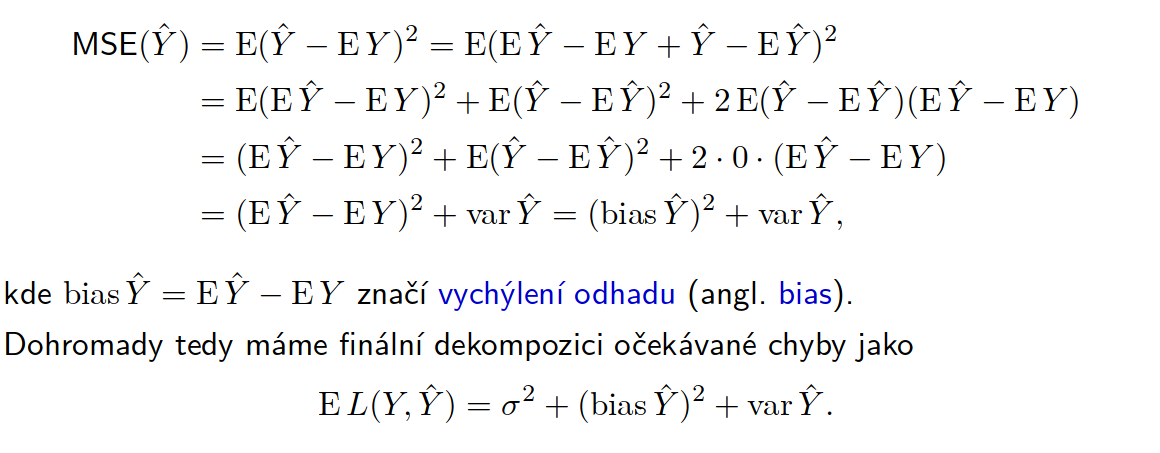
\includegraphics[width=\linewidth]{biasvariance}
\end{figure}


\begin{figure}
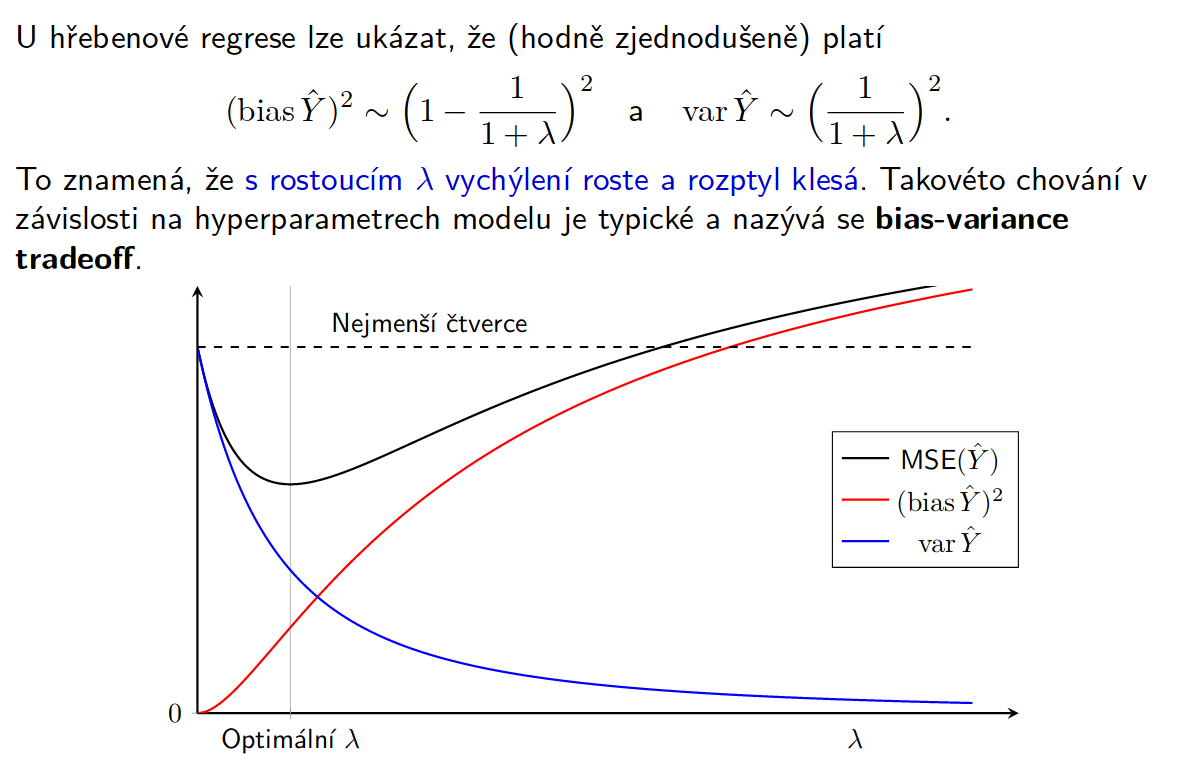
\includegraphics[width=\linewidth]{graph}
\end{figure}


\subsection{Extrémy funkce více proměnných}
\subsubsection*{Gradient}
\begin{theorem}
Buď $f:\mathbb{R}^d\rightarrow\mathbb{R}$ funkce $d$ proměnných, která má v bodě $a\in\mathbb{R}^d$ konečné všechny parciální derivace. Gredient funkce $f$ v bodě $a$ definujeme jako vektor
\begin{equation}
\nabla f(a)=\Big( \frac{\partial f}{\partial x_1}(a), \ldots, \frac{\partial f}{\partial x_d}(a) \Big).
\end{equation}
Označením $\nabla f$ pak myslíme gradient funkce jakožto zobrazení, které každému bodu, kde to lze, přiřadí gradient v tomto bodě.
\end{theorem}
Důležitou vlastností gradientu je, že ukazuje směr maximálního růstu funkce v daném bodě. 

\subsubsection*{Hessova matice}
\begin{theorem}
Buď $f:\mathbb{R}^d\rightarrow\mathbb{R}$ funkce $d$ proměnných. Hessovu matici funkce $f$ v bodě $a\in\mathbb{R}^d$ definujeme jako:

\begin{equation}
	H_f(a)=
	\begin{bmatrix}
   \frac{\partial^2 f}{\partial x_1^2} & \ldots &  \frac{\partial^2 f}{\partial x_1 \partial x_d}\\
   \vdots  & \ddots & \ldots\\
      \frac{\partial^2 f}{\partial x_1 \partial x_d} & \ldots &  \frac{\partial^2 f}{\partial x_d^2}
 \end{bmatrix},
\end{equation}
kde $\frac{\partial^2f}{\partial x_i \partial x_j}(a)=
\big(\frac{\partial}{\partial x_i}\big( \frac{\partial}{\partial x_j} \big)\big)(a)$ značí druhou parciální derivaci podle $x_j$ a $x_i$.
\end{theorem}

\begin{figure}[h]
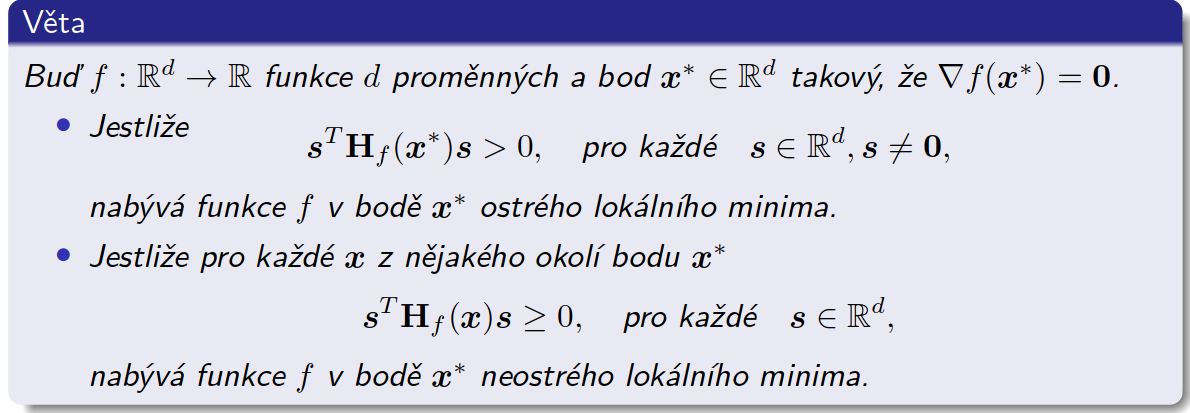
\includegraphics[width=\linewidth]{lokalni_extrem}
\caption{Existence minima}\label{pic:min}
\end{figure}






\end{document}

















